%% LyX 2.1.2 created this file.  For more info, see http://www.lyx.org/.
%% Do not edit unless you really know what you are doing.
\documentclass[english]{article}
\usepackage[T1]{fontenc}
\usepackage[latin9]{inputenc}
\usepackage{amsmath}
\usepackage{graphicx}

\makeatletter
\@ifundefined{showcaptionsetup}{}{%
 \PassOptionsToPackage{caption=false}{subfig}}
\usepackage{subfig}
\makeatother

\usepackage{babel}
\begin{document}

\section{Sensitivity to initial conditions}

As it was shown in the problem formulation the initial condition \ref{norm_initial}
assumes some existing fracture aperture and non zero length. One can
ask a question of what implications does the value of initial condition
have on solution. To answer this question a set of test scenarios
with various modifications to casual self similar start conditions
are presented. While some authors attempt to start form zero initial
width and opening, others take some known solution and treat it as
initial condition. The approach presented here uses the zero leak
off self similar solution given by Linkov\cite{MWL}, to identify
$w_{*}$and corresponding $l_{*}$. This values will be alternated
to show possible results of tempering with initial conditions. The
results will be presented as plots with multiple possible trajectories
of $L(t)$, each one corresponding to different values of $w_{*}$,$l_{*}$and
$a$ (which is initial time). As an example of such a plot consider
figure \ref{example_initial_plot} where several possible trajectories
of $L(t)$ are shown. 

Different initial values will affect the stability of computations.
The calculations which resulted in solver failures or incorrect fluid
balance value, relative loss of over $5\%$ of fluid, will be ignored
and not shown. All the tests will be carried out with initial time
vales of

\[
a=10^{-8},10^{-6},10^{-4},10^{-2},1
\]


and multiple values of some other parameters, giving in total of about
30-50 attempted fracture computations for each initial condition variation.

\begin{figure}
\centering\includegraphics[scale=0.4]{example_plot}\label{example_initial_plot}
\protect\caption{An example comparison of fracture lengths of three different fractures.
Despite different starting times $a$ and initial lengths all of the
trajectories want to behave initially as self similar solution and
eventually transits to large time asymptote.}
\end{figure}



\subsection{Self Similar solution and Large Time asymptotes}

In the paper by Linkov in\cite{MWL} the following self similar solution
is presented: 
\begin{equation}
w(t,x)=w_{n}h(x)^{1/3}(a+t)^{1/5},\quad h(x)=0.6\xi_{*}^{2}\sum_{j=1}^{j=\infty}\frac{b_{j-1}}{j}(1-x)^{j},\quad\xi_{*}=1.3208446(q_{0}/q_{n})^{0.6}.\label{self_similar_linkov}
\end{equation}


where fracture length, and consequently large time zero leak off asymptote,
is given by:

\begin{equation}
l(t)=\xi_{*}x_{n}(a+t)^{4/5}\label{eq:self_similar_l}
\end{equation}


The parameters $w_{n}$,$q_{n}$,$x_{n}$ depend on $k$ and $M$
values.

The large time asymptote for Carter Law was given by \cite{Nordgren}:

\begin{equation}
\frac{2q_{0}}{\pi}\sqrt{t}\label{eq:carter_law_large_time}
\end{equation}


A general equation for large time asymptote was derived by Perkowska
{[}???{]}, for pressure proportional Carter Law variant this results
in following large time asymptote:

\begin{equation}
\frac{q_{0}^{0.6}}{2}t^{0.4}\label{eq:pressure_carter_large_time}
\end{equation}



\subsection{Varying initial length}

Lets first examine the effect of changing the initial lengths. To
do so, the original initial crack length $l_{*}$ will be multiplied
by a factor $B$: 
\begin{equation}
\hat{l_{*}}=Bl_{*}
\end{equation}


Where the considered values of $B$ are:

\begin{equation}
B=10^{-5},\ 10^{-4},\ 10^{-3},\ 10^{-2},\ 10^{-1},\ 10^{0},\ 10^{1},\ 10^{2},\ 10^{3},\ 10^{4},\ 10^{5}.
\end{equation}


So now one can observe effects of changing just the fracture length.


\subsubsection{Zero leak-off}

Figure (\ref{length_zero_leak})

If there is zero leak-off starting from initial length bigger than
in self-similar formulation stops the fracture from growing in early
times as it takes longer to fill the crack with fluid. After that
time all fracture lengths tend to the same solution.

\begin{figure}[ht]
\begin{centering}
\includegraphics[scale=0.38]{L0_no_leak} 
\par\end{centering}

\protect\caption{Varying initial length - zero leak-off.}


\label{length_zero_leak} 
\end{figure}



\subsubsection{Carter leak-off}

Figure (\ref{length_carter_leak})

For Carter leak-off if the first variant of preconditioning (\ref{preconditioning_2}),is
used, the initial fractures tend to close vigorously at initial start
times grater than $10^{-2}$ if the fracture length was increased.
A number of attempts to start form larger times was effectively unsuccessful.This
problems were not encountered as much for the other variant of preconditioning
(\ref{preconditioning_1}), thous one can observe that computations
are generally easier if leak off is ignored for the initial opened
fracture length.

\begin{figure}[ht]
\begin{centering}
\includegraphics[scale=0.33]{L0_carter_leak} \includegraphics[scale=0.33]{L0_carter_leak_no_pre} 
\par\end{centering}

\protect\caption{Varying initial length - Carter leak-off. Left preconditioning variant
(\ref{preconditioning_2}), (\ref{preconditioning_1}) on the right.}


\label{length_carter_leak} 
\end{figure}



\subsubsection{Pressure Carter leak-off}

Figure (\ref{length_p_carter_leak})

Compared to the original Carter Law formulation ,the pressure proportional
leak-off does not handle extended lengths at initial times greater
than $10^{-2}$. 

Additionally curious case can be observed for $a=10^{-2}$ when a
fracture remains length function remains flat for a considerable amount
of time before joining the large time asymptote.

\begin{figure}[ht]
\begin{centering}
\includegraphics[scale=0.38]{L0_p_carter_leak} \includegraphics[scale=0.33]{L0_p_carter_leak_no_pre} 
\par\end{centering}

\protect\caption{Varying initial length - Pressure Carter leak-off. Left preconditioning
variant (\ref{preconditioning_2}), (\ref{preconditioning_1}) on
the right.}


\label{length_p_carter_leak} 
\end{figure}



\subsection{Varying the influx at crack mouth}

To analyze how perturbations of the influx at $x=0$ impact the solution
of the problem, lets multiply self-similar $q_{0}=1$ by a factor
$C$: 
\begin{equation}
\hat{q_{0}}=Cq_{0}
\end{equation}
with $\hat{q_{0}}$ a new influx. Here $C$ is in range

\begin{equation}
C=10^{-5},\ 10^{-4},\ 10^{-3},10^{-2},\ 10^{-1},\ 10^{0},\ 10^{1},\ 10^{2},\ 10^{3},\ 10^{4},\ 10^{5}
\end{equation}
It can be now compared how different pump-in rate change affect the
solution. It should be noted that in this scenario the large time
asymptote takes new value for each possible value of $C$.


\subsubsection{Zero leak-off}

Figure (\ref{q0_zero_leak})

\begin{figure}[ht]
\begin{centering}
\includegraphics[scale=0.38]{q0_no_leak} 
\par\end{centering}

\protect\caption{Varying initial influx - zero leak-off.}


\label{q0_zero_leak} 
\end{figure}



\subsubsection{Carter leak-off}

Figure (\ref{q0_carter_leak})

\begin{figure}[ht]
\begin{centering}
\includegraphics[scale=0.33]{q0_carter_leak} \includegraphics[scale=0.33]{q0_carter_leak_no_pre} 
\par\end{centering}

\protect\caption{Varying initial influx - Carter leak-off. Left preconditioning variant
(\ref{preconditioning_2}), (\ref{preconditioning_1}) on the right.}


\label{q0_carter_leak} 
\end{figure}



\subsubsection{Pressure Carter leak-off}

Figure (\ref{q0_p_carter_leak})

\begin{figure}[ht]
\begin{centering}
\includegraphics[scale=0.33]{q0_p_carter_leak} \includegraphics[scale=0.33]{q0_p_carter_leak_no_pre} 
\par\end{centering}

\protect\caption{Varying initial influx - Pressure Carter leak-off. Left preconditioning
variant (\ref{preconditioning_2}), (\ref{preconditioning_1}) on
the right.}


\label{q0_p_carter_leak} 
\end{figure}



\subsection{Varying the initial shape }

This time it will be investigated how the solution changes depending
on the initial shape of the fracture $w_{*}(x)$. Let us represent
the function as: 
\begin{equation}
\hat{w_{*}}(x)=A_{j}(1-x)^{\alpha_{j}},
\end{equation}
where $\alpha_{j}$ defines the shape of the initial fracture and
a constant $A_{j}$ is chosen so that the volume of the fracture is
the same for each initial shape.

The values of $\alpha_{j}$ are in range:

\begin{equation}
\alpha_{j}=-\frac{2}{3},\ -\frac{1}{3},\ 0,\ \frac{1}{3},\ 1,\ 2
\end{equation}



\subsubsection{Zero leak-off}

Figure (\ref{shape_zero_leak})

For a zero leak-off case, initial shape does not change behavior of
the solution. Depending on power $\alpha_{j}$ and initial time, the
length $L(t)$ may tend to the large fluid loss solution quicker than
for other values. If we start from lower value of $\alpha_{j}$, the
length of the fracture may stand still for some time and then start
growing only after it is filled with enough fluid. Nevertheless, eventually
all initial shapes will yield the same result.

\begin{figure}[ht]
\begin{centering}
\includegraphics[scale=0.6]{w0_no_leak} 
\par\end{centering}

\protect\caption{Varying initial shape - zero leak-off.}


\label{shape_zero_leak} 
\end{figure}



\subsubsection{Carter leak-off}

Figure (\ref{shape_carter_leak})

For Carter leak-off regime, after some time all initial shapes will
tend to the large fluid loss solution of $L(t)$, but for low values
of power $\alpha_{j}$ the fracture may recede until enough fluid
is pumped in to make the crack propagate. It it is caused by the fact
that more fluid leaks off to the formation than flows into the tip
region.

\begin{figure}[ht]
\begin{centering}
\includegraphics[scale=0.6]{w0_carter_leak} 
\par\end{centering}

\protect\caption{Varying initial shape - Carter leak-off. }


\label{shape_carter_leak} 
\end{figure}



\subsubsection{Pressure Carter leak-off}

Figure (\ref{shape_p_carter_leak})

When pressure proportional leak-off is used with starting time $a\leq10^{-2}$
obtained results are similar to those in zero leak-off case. 

\begin{figure}[ht]
\begin{centering}
\includegraphics[scale=0.6]{w0_p_carter_leak} 
\par\end{centering}

\protect\caption{Varying initial shape - Pressure Carter leak-off.}


\label{shape_p_carter_leak} 
\end{figure}



\subsection{Fractures with added linear extension to the initial shape}

For the last test initial condition modification lets consider if
the initial shape can be modified by addition of a long and thin extension
at the crack tip. After this modification the crack should have new
initial length:

\begin{equation}
\hat{l_{*}}=l_{*}(1+l_{extra}),\label{dzioby_L}
\end{equation}


where $\hat{l_{*}}$ is the new length, with addition of extra quantity
$l_{extra}>0$, that is a multitude of original length. Initial fracture
width changes as well, namely the old part obtained from self-similar
solution is squeezed along $x$-direction, while a linear function
covers amount contributed by $l_{extra}$. This change in initial
crack width can be written as:

\begin{equation}
\hat{w_{*}}(x)=\begin{cases}
w_{*}\left(x(1+l_{extra})\right) & \text{if }0\leq x\leq x_{*}\\
w_{*}\left(x(1+l_{extra})\right)\frac{1-x}{1-x_{*}} & \text{if }x_{*}<x\leq1,
\end{cases}
\end{equation}


Where $\hat{w_{*}}$is new initial shape, and $x_{*}$ is the connection
point:

\begin{equation}
x_{*}=\frac{1-\varepsilon}{1+l_{extra}},\label{xs}
\end{equation}


$\varepsilon$ a small value in $\varepsilon$-regularisation. 

To account for the change in preconditioning, the original used self-similar
length inverse is modified:

\begin{equation}
\hat{l}^{-1}=l^{-1}\left(\frac{x}{1+l_{extra}}\right).\label{dzioby_inverse}
\end{equation}


This new $\hat{l}^{-1}$ is later used to compute $\tau(x)$ in numerical
leak off scheme. The considered values of $l_{extra}$ are:

\[
l_{extra}=1,\ 25,\ 10,\ 20,\ 50,\ 100,\ 200
\]


Some examples of the effect of these extensions are presented in Figure
\ref{dzioby_piotrek}.

\begin{figure}[ht]
\begin{centering}
\includegraphics[scale=0.38]{dzioby_wykres} 
\par\end{centering}

\protect\caption{Aperture of fractures with added linear extension: $l_{extra}=0.5\ ,2,\ 8$.}


\label{dzioby_piotrek} 
\end{figure}



\subsubsection{Zero leak-off}

Figure (\ref{dzioby_zero_leak})

\begin{figure}[ht]
\begin{centering}
\includegraphics[scale=0.38]{dzioby_no_leak} 
\par\end{centering}

\protect\caption{Adding linear extension - zero leak-off.}


\label{dzioby_zero_leak} 
\end{figure}



\subsubsection{Carter leak-off}

Figure (\ref{dzioby_carter_leak})

\begin{figure}[ht]
\begin{centering}
\includegraphics[scale=0.38]{dzioby_carter_leak} 
\par\end{centering}

\protect\caption{Adding linear extension - Carter leak-off.}


\label{dzioby_carter_leak} 
\end{figure}



\subsubsection{Pressure Carter leak-off}

Figure (\ref{dzioby_p_carter_leak})

\begin{figure}[ht]
\begin{centering}
\includegraphics[scale=0.38]{dzioby_p_carter_leak} 
\par\end{centering}

\protect\caption{Adding linear extension - modified leak-off.}


\label{dzioby_p_carter_leak} 
\end{figure}



\subsection{Remarks on initial conditions}

One can observe that in the vast majority of successful computations
the outcome tends to the expected large asymptote regardless of applied
modifications to the initial conditions. This phenomena can be explained
by taking a closer look at figure(\ref{dzioby_aj}). Although the
initial shape is much different than what forms in most fracture simulations,
which generally closely resembles the lead asymptote $(1-x)^{\frac{1}{3}}$,
it can be observed that these fractures profiles adjust to resemble
this casual profile. Quite remarkably in both cases a new propagating
front can be observed appears as a fracture within other fracture.
This inside fracture (UDOWADNIAC ???) front itself propagates towards
the tip $x=1$, and is probably governed by an equation similar to
the speed equation (\ref{norm_speed}) used for main fracture front.
Interestingly, as shown by initial conditions variants with increased
fracture lengths, the fracture will not propagate significantly until
in fracture propagating front joins with the tip.

Another general observation is that a relation between the placement
of the initial starting point relative to starting small time asymptote
and the large time asymptote and general effectiveness of computational
scheme. These effects are shown on (\ref{initial_conditions_observations}).
Also note that as a general observed rule is, the longer the system
takes to solve, the more time the computation takes. The systems starting
in green regions would generally take less than 5 seconds to finish,
while other in yellow would take a multitude of that time, and the
one in red could fail after running for minutes.

\begin{figure}[ht]
\begin{centering}
\includegraphics[scale=0.38]{dzioby_aj} 
\par\end{centering}

\protect\caption{Evolution of profile for two fractures. }


\label{dzioby_aj} 

\subfloat[placeholder General observation on which initial condition combinations
allow for successful computations]{\begin{centering}
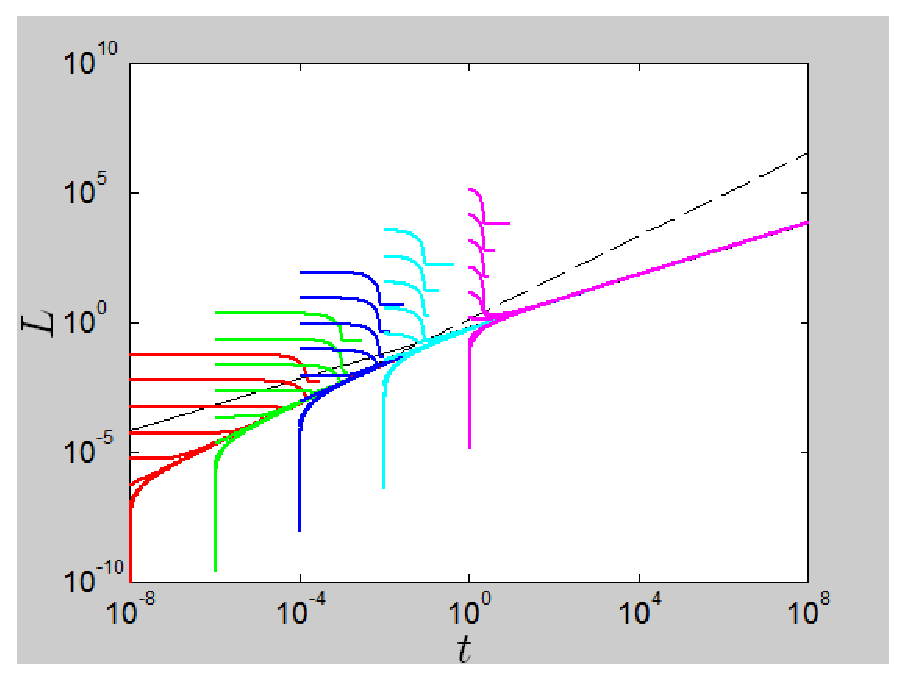
\includegraphics[scale=0.38]{broken} \includegraphics[scale=0.38]{\string"initial condition zones\string".eps} 
\par\end{centering}



\label{initial_conditions_observations} }
\end{figure}

\end{document}
